\section{Introduction}
Off-the-shelf Enrollment Systems are used by bigger universities in the Philippines while universities with smaller populations usually develop their own systems in-house. What is common with these systems is that their continued usage introduces a different set of problems for users coming from different backgrounds and technical proficiency. In general, most enrollment systems both off-the-shelf and developed in-house would be made to address common problems encountered in enrollment. Such issues would revolve around managing different block schedules, accommodating irregular students, allocating logistics such as classrooms, computer laboratories and field rooms, and assigning faculty. These tasks are usually pre-enrollment activities that are done in preparation for actual enrollment. Aside from this, there are other systems and modules that cater to the other stages of the Enrollment and Post-Enrollment Process. Regardless of the stage of enrollment concerned, human collaboration is an important aspect that is seldom considered when designing and developing key systems and features. As a matter of fact, even systems that have partial automation still require the human element especially when involved with key major decisions and time-pressed concerns. In Pre-enrollment activities alone, constant collaboration, communication and clarification is essentials towards the successful planning of enrollment in a given university. Users from varying levels and organization scope, who are involved in these stages are key decision makers who can implement changes in enrollment that will definitely affect the academic load of both faculty and students. 

In comparison, these systems are not entirely interactive and collaborative in nature. For key officials who are newly-placed into their posts, an additional learning curve prolongs the process. Most especially for off-the-shelf systems, they provided limited user feedback and do not give an avenue for collaboration between other key personnel involve. As such, these systems may generally hinder collaboration. To some organizations and universities, the collaborative aspects in the process of enrollment are relied from the usage of third-party tools such as Viber, Messenger, and other messaging platforms. These systems do not also give its current users insights on which portion of the work or process are being worked on by other key staff and personnel. As a result, either a feature may be locked to a certain user for a given moment or two users might be inputting conflicting information that could have been avoided if these users are aware of what they are both editing. The visual interface of these systems must be accompanied by design elements that guide all of its users towards understanding the process and the impacts of the changes they apply in the enrollment system. Our work makes an inquiry into the underlying design factors that affect the collaborative behaviors in enrollment and timetabling systems, specifically in the pre-enrollment process. We sought to understand the human factors involving key users and administrative personnel when operating an in-house designed software prototype with key collaborative features in supporting pre-enrollment. We did a formative study composed of interviews, observations, user tests with participants. We developed a prototype based on these findings which we iteratively tested as well. In this paper we: (1) Observe and understand how key personnel from a specific university, collaborate in pre-enrollment. We also (2) derive and formulate guidelines towards a collaborative online platform that these key personnel can use in planning their pre-enrollment deliverables such as course schedule, faculty schedule and block schedules. Additionally, we (3) discuss design implications for supporting these collaborative activities. Lastly, we (4) reflect on how we can design better enrollment systems that foster collaboration between key staff, and towards pushing it in different stages of the enrollment process. 

\section{Related Work}
\subsection{Academic Timetabling Systems}
The Automated Scheduling System (ASSYST) \cite{Assyst} was developed to automate the course scheduling process. It had two modules for each user type: the College Academic Assistant (CAA) module and the Chair/Vice-Chair module. \cite{Assyst} generates an initial course schedule and improves it through Genetic Algorithms. ASSYST ver. 2 \cite{Assyst2} extended features of its predecessor to include faculty scheduling. The faculty schedules were also generated using Genetic Algorithms. A web-version of the system was developed after several years, named e-ASSYST \cite{eAssyst}. Unlike its predecessors, it used Tabu Search to create faculty schedules. 

\cite{2013Nigeria} developed a timetabling system that utilizes Constraint-Satisfaction techniques to automate their timetabling process. The system was able to quickly generate lectures schedules that satisfied both soft and hard constraints given to it, and was successfully tested using the System Usability Scale method. \cite{UPM} is another web-based system that aimed to expedite creating course schedules for their departments following the specified constraints of the user. It boasted the ability to generate a timetabling schedule in the case an incomplete solution is found. \cite{Oprea2007} developed a timetabling system that operates through Multi-Agent Systems. The agents negotiate with one another in the case of conflicts, and help each other to form an optimal or sub-optimal timetabling schedule. \cite{bulacanState}, meanwhile, addressed the decentralization of resources from university parent and satellite campuses. The system aids users assigned to create faculty and course schedules. The system was only designed to help evenly distribute the resources between university campuses through a centralized database system that stores university resources to guide its users in creating schedules. \cite{UniTime} is a commercial timetabling system that hosts multiple useful features such as: timetable creation, editing timetables, schedule conflict prevention, and room allocation. \cite{UniTime} also allows multiple ways to create the class schedules, offering centralized, distributed and hybrid approaches. It provides options for the users to customize the schedule, satisfying hard constraints imposed on the course scheduling process by departmental rules.

The focus of \cite{Assyst, Assyst2, eAssyst, UPM, bulacanState, 2013Nigeria, Oprea2007, UniTime} have been towards automating the creation of course schedules and improving these generated schedules with optimization algorithms. However, most of these systems omit the human collaboration component that is essential in the enrollment process. For instance, \cite{Assyst} and \cite{Assyst2} have modules for each user type but it does not support collaboration between them. \cite{arrowSmith}, meanwhile, takes a more humanist approach and tackled the usability of academic timetabling systems. The course and faculty scheduling features remain but it does not rely on an optimization algorithm to create and improve these schedules. Their system focused, instead, on improving its user interface design by following a set of heuristics by \cite{Paz}. It was also verified iteratively through Keystroke-Level Modeling. Despite the change of focus, \cite{arrowSmith} also did not address human interaction and collaboration in their design and testing phases. Thus, collaboration within timetabling systems remains unexplored. This can put a damper towards deploying these systems to the involved personnel as collaboration is important when executing these processes. \cite{arrowSmith}, though, is in the right direction; its humanist approach lends itself to focusing on enhancing the user's interactions with the system. Nevertheless, collaboration is still lacking and therefore a factor to be considered.

% Discuss here the previous CCS systems such as ASSYST, ASSYST2, E-ASSYST, ArrowSmith etc. In the discussion, lets not mention DLSU. Lets mention how these systems were developed and what was their focus. Then conclude by saying, was collaboration a key issue. what key features of these systems worked and did not work and will work or used for assystx. 

\subsection{Collaboration Systems}
%\cite{Dix:2003:HI:1203012} talks about email as a good example of a CSCW system. Originally based on the conventional postal system, it allows communication between individuals who are at physically removed locations from each other. A user can create an email and send it to another person or a group of people. When a person receives the email, a notification would pop up to prompt the receiving person that a new email has just arrived. The email can be then viewed and the user may respond accordingly to its contents.

\citep{googleDocs} is a proprietary online word processing application that allows users to write, edit, and collaborate on documents. The application boasts several collaborative features such as: document sharing, concurrent editing, online chat, and comments. It allows both asynchronous and synchronous collaboration between users in a single document. Asynchronous because user do not have to be working at the same time frame to write the document, and synchronous because it allows real time functions such as concurrent editing, and the chat features. \cite{googleSheets} is a proprietary online spreadsheet application which allows users to create, edit, and collaborate on spreadsheets. The application also boasts the same collaborative features as \cite{googleDocs} and can also accommodate both asynchronous and synchronous collaboration. The two applications are for general use; it can be used for timetabling processes. However, timetabling requires a tailored application to fully capture its needs and intricacies, for example a feature for scheduling wherein the application can check for redundancies and errors. Thus, \cite{googleDocs} and \cite{googleSheets} cannot fully function as a timetabling application. The collaborative features of concurrent editing and messaging were used as inspiration for ASSYSTX's implementation. 

%The Google Calendar API is a tool that allows developers to add features that allow users to manage their respective calendar events\citep{googlecalendar}.  
%Slack is marketed as a collaboration hub and tool that allows users to manage their respective conversations \citep{slack}. The application makes use of channels that segregate a user's respective task, team, or anything that is relevant to the user. Collaborative channel functions include: message sending in the channel, a join-share function, a leave function, voice and video calls, screen-sharing, and file sharing. The application allows asynchronous collaboration as it does not require users to be online at the same time for its messaging, join-share, leave, and file sharing features. It also allows synchronous collaboration as users have to be online for its video call, screen-sharing, and also in its chat function.

%Trello is a project management collaboration tool that allows teams to keep track of progress in their projects \citep{trello}. The application makes use of a board that holds a collection of lists that represent project tasks and elements. Lists are filled with cards that represent a unit that is associated with the list. Collaborative features include: Adding of members to a Trello board, adding members to a card, card checklist and due dates, file sharing via attachments, comments, notifications, and real time board syncing. The application allows asynchronous collaboration as members do not have to be online to access any of the collaborative features. 

%Look at other related work outside dlsu put them here. same guide questions. 

\section{Methodology}
The methodology follows the Design Research approach as seen in the works of \cite{deja2018myosl, deja2018flow, chan2019applying}. It approaches a user-centric methodology where user needs are extracted and transformed into features that are intended for the use-case concerned. It is followed by a prototyping phase that allows the study to be iterated and tested by the intended users before actual deployment. More details are seen as described in Fig \ref{fig:pipelinediagram}. 
\begin{figure}[h]
   \centering
   \includegraphics[scale=0.18]{Diagrams/Methodology.png}
   \caption{The research methodology for ASSYSTX. The first phase (P1) dealt with understanding the stakeholders' needs and issues in the course scheduling and faculty load assignment processes. The second phase (P2) used the data to be gathered from the first to design and develop the existing system. The third phase (P3) involved repeatedly testing and validating the newly developed system with the stakeholders.}
    \label{fig:pipelinediagram}
\end{figure}

% hello
% Insert here the research framework (un diagram)

\subsection{Needfinding and User Research}
Stakeholder interviews and timetabling demonstration comprise the first phase, as it follows the Interaction Design process described in \cite{Dix:2003:HI:1203012}. The purpose is to gain a better understanding of the timetabling processes. The stakeholders involved are the Academic Programming Officer (APO), who is in charge of course scheduling, and the Department Chairs and Vice-Chairs, in charge of faculty scheduling. Informed consent was secured before conducting the interviews and demonstration.

The following questions were asked during the interviews:
\begin{enumerate}
    \item How is course scheduling done? What are its difficulties?
    \item How is faculty load assignment done? What are its difficulties?
    \item How do you prioritize who should input data first when collaborating?
    \item How do you communicate with the other stakeholders, i.e. Chairs, Vice Chairs, APO, etc.?
    \item What are some features you would like to see in a timetabling application?
\end{enumerate}

Follow-up questions were also asked depending on the stakeholder's answers and roles. Afterwards, a demonstration of the timetabling process is performed by the involved stakeholder. While in action, additional questions were also asked for clarity. Data collated -- interview answers and observations -- were processed into possible solutions to define the needs and issues of the stakeholders. These were then proposed to the stakeholders with the goal of garnering comments and suggestions. This process was repeated until both stakeholders and researchers were satisfied with the solution.

\subsection{Iterative Prototyping}
The initial prototypes followed the seven principles that summarizes user-centered design process \cite{Norman:2002:DET:2187809}. We came up with different prototypes for possible solutions to present with the stakeholders. The stakeholders also explored the previous Arrowsmith system to provide suggestions for improvements in line with the prototypes. Once we had finalized and agreed upon the interface design, we proceeded to development. Getting the user interface to be understandable and easy to use was a priority at this phase. As such, we followed the interface and visual design principles of \cite{Soper2016, Gong2009, Thimbleby}. For interface validation, we used the heuristics set by \cite{Paz}. We developed a high-fidelity prototype that allowed the stakeholders to interact with the system and perform timetabling processes. The iterations were used to help in garnering feedback about the prototype, if it was a usable, full-fledged application. We had a total of three (3) iterations of development.

\begin{figure}[h]
   \centering
   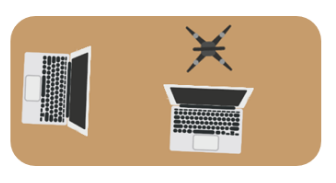
\includegraphics[scale=1.0]{Diagrams/Test_Setup.PNG}
   \caption{The Test Setup for the Iterative Usability Testing. Qualitative data were collected through audio and video recordings (represented by the tripod) of the stakeholders. The computer on the left side is used to take notes and record the initial observations during the tests. The post-survey test was also conducted in this computer. The computer on the right side is for the prototype system. When testing involves two stakeholders, they are positioned far from each other.}
    \label{fig:pipelinediagram}
\end{figure}

\subsection{Iterative Usability Testing}
Usability tests were performed to determine the prototype's effectiveness as a usable and collaborative timetabling application. These were conducted in an environment wherein audio and visual disturbances were at a minimum. The participants were the stakeholders, the APO and a Department Vice-Chair. Consent forms were provided before the respective tests. After they have given their consent, we oriented them with our goals and their tasks for the tests. They were also encouraged to follow a think-aloud protocol for us to collect their thought process throughout. The stakeholders performed tasks depending on their real-life roles, course scheduling for the APO and faculty loading for the Vice-Chair, within the prototype system. We also had a total of three (3) iterations for usability testing. 

The first iteration focuses on the gathering of feedback about the interface itself. The task completion test was primarily designed to check if the system follows usability heuristics for good user interfaces. This iteration also investigates how to improve the interaction design of the system. Completed tasks are represented through a scoring system of 1 - 3: Accomplished being the highest score (3), Accomplished but with difficulty (2) representing the middle score, and Failed (1) as the lowest score. The tasks can be found in Table \ref{tab:tasks1}.

\begin{table}
  \centering
  \caption{Iteration 1 Tasks}~\label{tab:tasks1}
  \addtolength{\tabcolsep}{2pt} 
  \begin{tabular}{p{0.5cm}|p{6.5cm}}
  	\toprule
    \rule{0pt}{8pt}No. & Task \\[2pt]
    \toprule
    T1 & Find the place in the website where all the offerings are listed \\
    T2 & Modify a course offering \\
    T3 & Add a new course offering \\
    T4 & Know where to find how to send concerns and where to find received concerns \\
    \bottomrule
  \end{tabular}
  \addtolength{\tabcolsep}{-2pt} 
\end{table}

The second iteration of testing gave emphasis on the functionality of the timetabling features of the system. The testing aimed to confirm if the system improved compared to the previous iteration, validate its effectiveness, and further improve the interaction design. The completion task followed the same scoring system from the previous iteration. The tasks are listed at Table \ref{tab:tasks2}. To help in finding these results, we administered a post-test survey for the participants to accomplish. This will also help us further understand what the participant had experienced in using the system. As seen in Table \ref{tab:scoring_scheme}, the results from the survey are answered on a scale of 1 - 4, with 1 (Strongly Disagree) being the lowest, and 4 (Strongly Agree) being the highest. The questions for the survey can be found in Table \ref{tab:itr2_questions}. 

\begin{table}
  \centering
  \caption{Iteration 2 Tasks}~\label{tab:tasks2}
  \addtolength{\tabcolsep}{2pt} 
  \begin{tabular}{p{0.5cm}|p{6.5cm}}
  	\toprule
    \rule{0pt}{8pt}No. & Task \\[2pt]
    \toprule
    T1 & Modify course offering and check if changes made by another role are saved. \\
    T2 & Deload a Faculty \\
    T3 & Raise concerns and receive concerns from another role \\
    T4 & Track the changes made through revision history \\
    \bottomrule
  \end{tabular}
  \addtolength{\tabcolsep}{-2pt} 
\end{table}

\begin{table}
  \centering
  \caption{Post-Test Survey Scoring Scheme}~\label{tab:scoring_scheme}
  \addtolength{\tabcolsep}{2pt} 
  \begin{tabular}{p{1cm}|p{5cm}}
  	\toprule
    \rule{0pt}{8pt}Score & Definition\\[2pt]
    \toprule
    4 & Strongly Agree \\
    3 & Agree \\
    2 & Disagree \\
    1 & Strongly Disagree \\
    \bottomrule
  \end{tabular}
  \addtolength{\tabcolsep}{-2pt} 
\end{table}

The third iteration of testing focused on the collaboration between users. Both stakeholders were present in the same room and both simultaneously used the prototype. However, verbal communication was restricted. The test was designed to validate if multiple users can accomplish their tasks successfully and collaboratively. The tasks of the participants for this iteration can be found in Table \ref{tab:tasks3}. For this specific test, a 0 - 4 scoring scheme was used. The corresponding definition of each score can be found in Table \ref{tab:itr3_scoring_scheme}. Similar to the previous iteration, a post-test survey was also administered. The questions are similar from the previous testing, as seen in Table \ref{tab:itr2_questions}, so that we can see if there are changes in the answers of the participants. 

\begin{table}
  \centering
  \caption{Iteration 3 Tasks}~\label{tab:tasks3}
  \addtolength{\tabcolsep}{2pt} 
  \begin{tabular}{p{0.5cm}|p{6.5cm}}
  	\toprule
    \rule{0pt}{8pt}No. & Task \\[2pt]
    \toprule
    T1 & Successfully create and modify a course across all users \\
    T2 & Check if changes made by a user reflects to the other user \\
    T3 & Raise concerns to the concerned user \\
    T4 & Track changes made by all users \\
    \bottomrule
  \end{tabular}
  \addtolength{\tabcolsep}{-2pt} 
\end{table}

\begin{table}
  \centering
  \caption{Iteration 3 Test Scoring Scheme}~\label{tab:itr3_scoring_scheme}
  \addtolength{\tabcolsep}{2pt} 
  \begin{tabular}{p{1cm}|p{5cm}}
  	\toprule
    \rule{0pt}{8pt}Score & Definition\\[2pt]
    \toprule
    4 & Accomplished Easily \\
    3 & Accomplished but with Confusion \\
    2 & Accomplished but Assisted \\
    1 & Accomplished by Mistake \\
    0 & Did not accomplish \\
    \bottomrule
  \end{tabular}
  \addtolength{\tabcolsep}{-2pt} 
\end{table}

\begin{table}
  \centering
  \caption{Criteria Used for Evaluating Collaboration}~\label{tab:itr2_questions}
  \addtolength{\tabcolsep}{2pt} 
  \begin{tabular}{p{.5cm}|p{2.75cm}|p{.5cm}|p{2.70cm}}
  	\toprule
    \rule{0pt}{8pt}No. & Task & No. & Task\\[2pt]
    \toprule
    Q1 & I am able to share my work with a person from a different role &  Q12 & I am able to track which person made what changes quickly\\
    Q2 &  I am able to see the work of a person from a different role  & Q13 & I am able to raise concerns to a person from a different role quickly\\
    Q3 & I am able to track which person made what changes & Q14 & I am able to receive concerns from a person from a different role quickly\\
    Q4 & I am able to raise concerns to a person from a different role & Q15 & I can collaborate with the other role through the system quickly\\
    Q5 & I am able to receive concerns from a person from a different role & Q16 & I am able to share my work with a person from a different role easily\\
    Q6 & I can collaborate with the other role through the system & Q17 & I am able to see the work of a person from a different role easily\\
    Q7 & I can easily see the contents of the system & Q18 & I am able to track which person made what changes easily\\
    Q8 & I can easily find what I'm looking for in the system & Q19 & I am able to raise concerns to a person from a different role easily\\
    Q9 & Everything I need to do my tasks are available  & Q20 & I am able to receive concerns from a person from a different role easily\\
    Q10 & I am able to share my work with a person from a different role quickly & Q21 & I can collaborate with the other role through the system easily\\
    Q11 & I am able to see the work of a person from a different role quickly & & \\
    \bottomrule
  \end{tabular}
  \addtolength{\tabcolsep}{-2pt} 
\end{table}

Feedback gathered were both qualitative and quantitative data. Qualitative data came from interviews and audio-video recordings. The video recordings used includes a face camera to observe the facial expressions of the testers and the screen-capture of the system-interactions made by the testers during the test. Figure \ref{fig:cvc_testing} shows a screenshot of the face camera of the vice-chair tester along with the screen-capture. Quantitative data was procured from the \textit{Task Completion Test Scores} and \textit{Post-Test Surveys} that the users were asked to answer after an iteration task test. 


% Insert here figures describing the UT setup
\begin{figure*}[]
\centering
   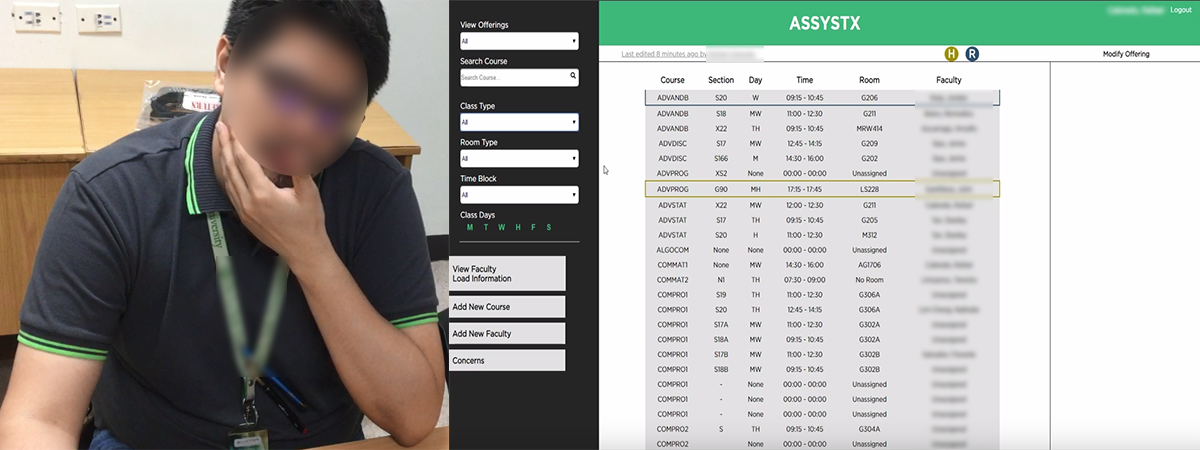
\includegraphics[scale=1.5,keepaspectratio]{PCSC2019_latex/Tests/sirTighe.png}
   \caption{Testing: The computer's face camera captures reactions of the participant while also capturing what he sees on the screen while using the system}
    \label{fig:cvc_testing}
\end{figure*}
% Guide questions, objectives discussions

\section{Results and Findings}
hello
\subsection{System Design}

\begin{figure}[h]
   \centering
   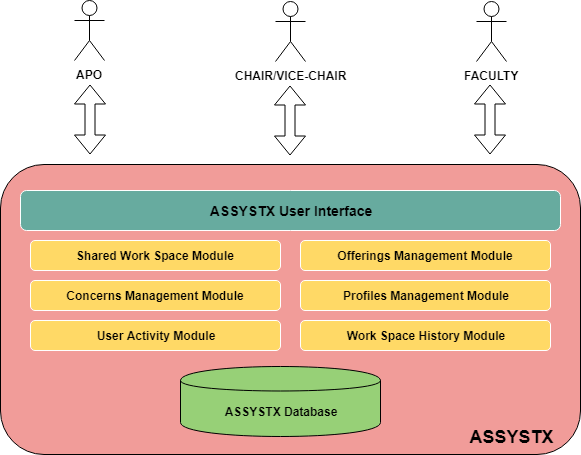
\includegraphics[scale=0.4]{Diagrams/System_Architecture.png}
   \caption{ASSYSTX System Architecture. The ''Shared Work Space" module allows users to collaborate through the interface to access the other modules such as ``Concerns Management" and ``Work Space History" modules to create a course schedule}
    \label{fig:pipelinediagram}
\end{figure}

There are a total of six modules in ASSYSTX. The \textit{Shared Work Space Module} enables the users to use the system with a graphical user interface. The module is also responsible in creating the shared work space for the users to collaborate into when performing their respective tasks. The \textit{Offerings Management Module} handles all features relating to the course offerings list. The module handles creating a course offering; changing its status; assigning a time slot, room, and faculty; and dissolving an offering. Conflict resolution and rule violation checking when assigning a room or faculty are also implemented within this module. Similar to the \textit{Offerings Management Module}, the \textit{Profiles Management Module} handles all features for course and faculty profiles. These profiles are used for creating a course offering. Thus, this module is responsible for the creation and management of courses and faculty. Faculty deloading is also performed under this module. \textit{Concerns Management Module}, meanwhile, is responsible for raising and receiving concerns. This module ensures that the concerns reach the target receiver. Acknowledgement and notifications also fall under this module. The \textit{Work Space History Module} is in-charge of auditing the changes made in the course offerings list of the system. These logs are then relayed to the \textit{User Interface Module} for display in the work space. Lastly, the \textit{User Activity Module} tracks the user's actions within the system. The module records the course offering currently being modified, the user's last seen concern and change log. These are used for notifications and help in inciting collaboration within the work space.

% Insert here the system design 
% Insert here key screenshots of the live edit, the send message feature
\begin{figure*}[h]
   \centering
 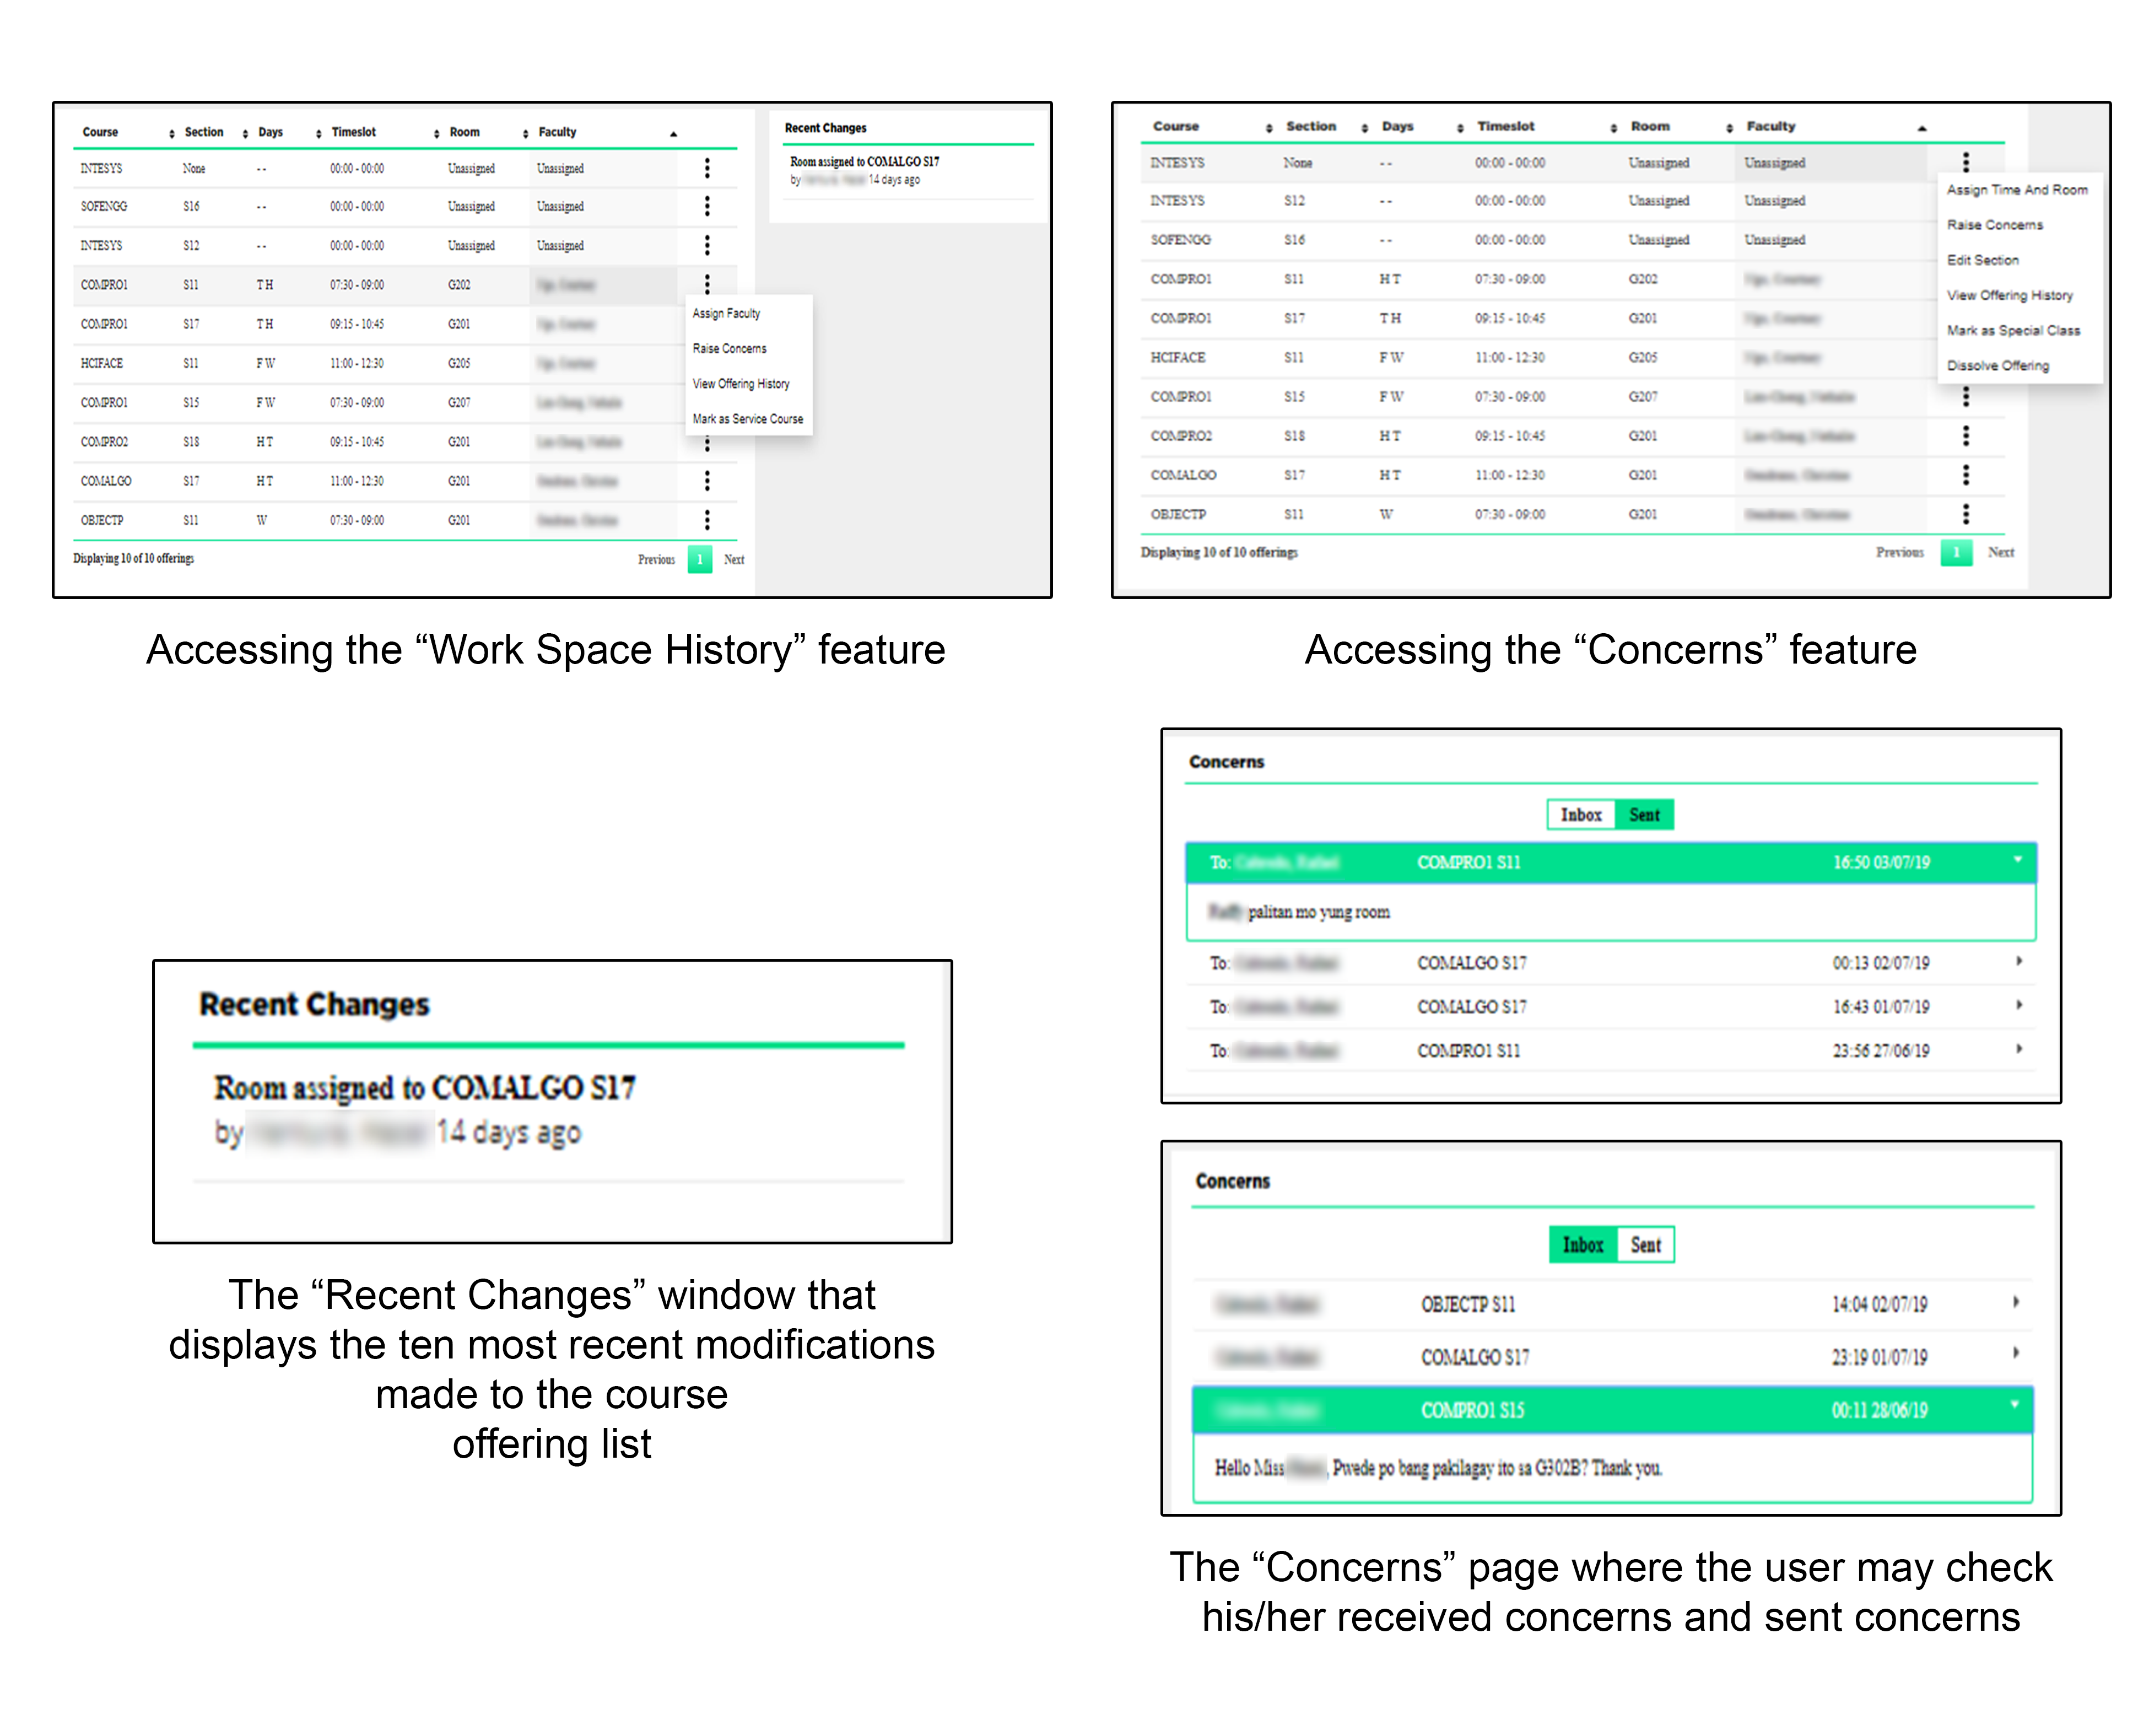
\includegraphics[width=\textwidth,height=\textheight,keepaspectratio]{PCSC2019_latex/Screenshots/assystxScreenshots.png}
   \caption{Two of the ASSYSTX Collaborative Features: Work Space History and Concerns} \label{fig:assystxScreenshot}
\end{figure*}

% Insert here other features of the software
% discussion sya ng key majors 

\subsection{Usability Tests}
% Insert here UT results (table)

% Insert here table comparing the UT scores
A summary of scores, divided per each cluster, can be found at Table \ref{tab:summarized_post_test_cluster}. It can be observed from the table that the average rating per cluster improves as the iterations go on. This can imply that there are improvements in the user experience of the system. With the \textit{Collaborative Features} cluster having improved the most, followed by the \textit{Speed} cluster, \textit{Ease of Use}, and finally \textit{Accessibility}. The increase in the \textit{Collaborative Features} cluster may be attributed to the fact that the improvements on the collaborative features, especially the raising of concerns, which allows users to communicate , negotiate, and plan out what is needed next for the schedule. Compared to the previous iteration, the participants were able to easily utilize the concerns feature. Improvements in the Work Space History, which allows users to check on the progress made by other users to guide them in their next courses of action can also be credited for the increase. 

In order to validate whether the rise in scores were significant enough for each cluster, We performed hypothesis testing between the two iterations' scores. The following null and alternative hypotheses are: 
 \label{list:significance_testing}
 \begin{itemize}
    \item $H_0$ - There is no significant difference between the mean scores of Iteration 2 and 3 per cluster.
    \item $H_\alpha$ - There is a significant difference between the mean scores of Iteration 2 and 3 per cluster.
\end{itemize}

The sample size was identified through t-statistic, or total number of questions, are less than 30. Lastly, the significance value will be 5\% or 0.05. If the computed p-value is less than 0.05, then the null hypothesis can be confidently rejected and accept the alternative hypothesis. The results of the hypothesis testing can be seen at Table \ref{tab:summarized_significance_testing}.

Three clusters, Collaborative Features, Speed, and Ease of Use, had a p-value of less than 0.05, indicating a significant difference in the scores. While the scores of the Accessibility cluster itself had improved, it remains to be the lowest-scored cluster and not having much significant difference. This may be due to lack of prompts and call to action to guide the user in the system. The unfamiliarity of the participant to system may also be attributed to this.

\caption{\label{tab:summarized_post_test_cluster}Summarized Post-Test Survey Cluster Scores from Iteration 2 - 3}
\begin{table}
\centering
\caption{\label{tab:summarized_post_test_cluster}Summarized Post-Test Survey Cluster Scores from Iteration 2 - 3}
\begin{tabular}{|l|l|l|l|l|l|l|}
\hline
\textbf{Cluster} & \textbf{I2} & \textbf{I3} & \mu & \textbf{I3 - I2} \\\hline
Collaborative Features & 3.00 & 3.75 & 3.40 & 0.75\\\hline
Accessibility & 2.67 & 3.00 & 2.80 & 0.33\\\hline
Speed & 3.00 & 3.58 & 3.30 & 0.58\\\hline
Ease of Use & 3.00 & 3.67 & 3.30 & 0.67\\\hline
Average &  &  &  & 0.58\\\hline
\end{tabular}
\end{table}

\begin{table*}
\centering
\caption{\label{tab:summarized_significance_testing}Summarized Significance Testing Results}
\resizebox{15cm}{!}{\begin{tabular}{|l|l|l|l|l|l|l|}
\hline
\textbf{Cluster} & \textbf{I2 Mean} & \textbf{I2 St.Dev.} & \textbf{I3 Mean} & \textbf{I3 St.Dev} & \textbf{t-statistic} & \textbf{p-value}  \\\hline
C1. Collaborative Features   & 3.000 & 0.000  & 3.750 & 0.250 & 7.348 & 0.000  \\\hline
C2. Accessibility            & 2.667 & 0.471  & 3.000 & 0.000 & 1.225 & 0.374 \\\hline
C3. Speed                    & 3.000 & 0.000  & 3.580 & 0.344 & 4.159 & 0.004 \\\hline
C4. Ease of Use              & 3.000 & 0.000  & 3.667 & 0.236 & 6.928 & 0.000 \\\hline
\end{tabular}}
\end{table*}
\begin{figure}[h]
   \centering
   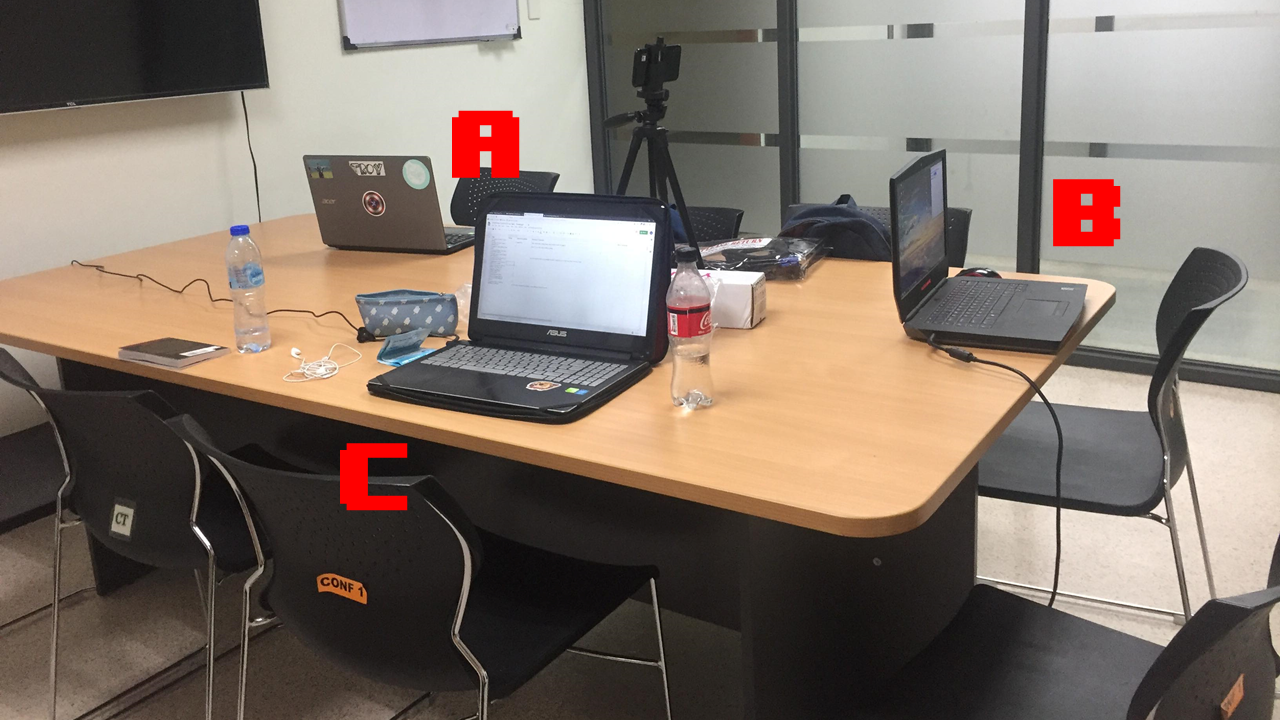
\includegraphics[scale=0.2]{PCSC2019_latex/Tests/test_setup_iteration3.png}
   \caption{Iteration 3 Test Setup}
    \label{fig:itr3_testsetup}
\end{figure}

\subsection{Human-Human Collaboration Factors}
Stakeholders must work together to create an agreeable schedule for a given term, taking into account variables that are present for that specific term. The APO preempts the process through creating a list of course offerings based on the college's flowcharts and batch size. Then she proceeds to assign a room and time slot for the course offerings. The APO may create more offerings following a request from the Chairs/Vice-Chairs. The Chairs/Vice-Chairs, meanwhile, are in-charge of assigning faculty to the course offerings. Criteria for assigning faculty include past teaching experiences with a certain course, his/her areas of expertise, and his/her current work load. Faculty may request to the APO about assigning specific time slots on specific offerings to ascribe to their planned faculty assignment. This may or may not be followed by the APO.


In the last iteration, the college APO and the Software Technology Vice-Chair were asked to test the system. The test setup can be seen in Figure \ref{fig:itr3_testsetup}, wherein the vice-chair was seated in position `A', the APO in `B', and a designated data-logger in `C' that would observe the progress and reactions of both parties. The APO created a course offering and had assigned a room to it. The vice-chair then assigned a faculty member to that course. The APO attached a concern to a course offering which the vice-chair acknowledged.


\textit{Human-Human Collaboration} allows multiple stakeholders to contribute and coordinate in handling the factors in creating the schedule. The APO who is responsible for providing the courses needed to be offered in the term will need to coordinate with the Chairs responsible for loading the faculty inside those courses. In assigning the faculty of a given course, there might be a need to change its properties (e.g. time slot, room assigned) in order for it to conform to his/her needs.


\subsection{Human-Computer Collaboration Factors}
The ASSYSTX system acted as the collaboration tool for the CCS timetabling process. In the last iteration, it acted as the medium where the APO and vice-chair testers simulated the timetabling process. When the APO had created a new course offering, the vice-chair was easily able to find it, which enabled him to load a faculty to the course with ease. Similarly, the APO was able to verify that the vice-chair had assigned a faculty member to the course offering she created. When the APO had attached a concern to another course offering, the vice-chair was able to receive it and acknowledge the concern. 

The system provided an avenue where users may perform the basic timetabling tasks such as creating course offerings and modifying an existing course offering to facilitating the collaboration between users. The system regularly updates the course offerings and concerns such that the users may act faster with their pending tasks. It also makes a record of changes, through both the ``Offering History" and ``Recent Changes" features such that the users may keep track of what they have done and what others have done so that they may make plans on their next courses of action. 

In \textit{Human-Computer Collaboration} there is a clear division of work between the user and the system. In the context of timetabling, the actual manipulation of courses and faculty are handled by the users, while the system only assists. It allows for multiple users to synchronously work on the schedule without conflicts. The system also acts as a ``rule-checker" that examines whether the schedule conforms to rules that are set by the college (e.g. faculty teaching loads, time-slot conflicts).  

\section{Conclusion and Future Work}
We were able to iteratively develop a collaborative timetabling application through ASSYSTX. Feedback after tasks was the general weakness of the system, as it hampered the accessibility of the system, both qualitatively and quantitatively. The collaborative features received the highest average score, albeit based off one test. All the tasks were accomplished by both participants and were done collaboratively in the third iteration. The participants did not deviate from the actual timetabling process (e.g. APO creates offering and assigns time and room before Vice-Chair assigns faculty) in all three iterations. The third iteration version of the system does allow both participants to modify the same course offering, however this was not explored nor considered.

For future work, testing the system through more conflict-driven situations that requires collaboration is a must. The tests we performed only concerned with the collaborative features' functionality, not necessarily its effectiveness in difficult situations. There is also a need to perform tests with more than two participants. A speed metric for comparison between performing tasks with and without the collaborative features can also help improve the system's performance.

\begin{comment}
\subsubsection{Inline (In-text) Equations}
A formula that appears in the running text is called an
inline or in-text formula.  It is produced by the
\textbf{math} environment, which can be
invoked with the usual \texttt{{\char'134}begin\,\ldots{\char'134}end}
construction or with the short form \texttt{\$\,\ldots\$}. You
can use any of the symbols and structures,
from $\alpha$ to $\omega$, available in
\LaTeX~\cite{Lamport:LaTeX}; this section will simply show a
few examples of in-text equations in context. Notice how
this equation:
\begin{math}
  \lim_{n\rightarrow \infty}x=0
\end{math},
set here in in-line math style, looks slightly different when
set in display style.  (See next section).

\subsubsection{Display Equations}
A numbered display equation---one set off by vertical space from the
text and centered horizontally---is produced by the \textbf{equation}
environment. An unnumbered display equation is produced by the
\textbf{displaymath} environment.

Again, in either environment, you can use any of the symbols
and structures available in \LaTeX\@; this section will just
give a couple of examples of display equations in context.
First, consider the equation, shown as an inline equation above:
\begin{equation}
  \lim_{n\rightarrow \infty}x=0
\end{equation}
Notice how it is formatted somewhat differently in
the \textbf{displaymath}
environment.  Now, we'll enter an unnumbered equation:
\begin{displaymath}
  \sum_{i=0}^{\infty} x + 1
\end{displaymath}
and follow it with another numbered equation:
\begin{equation}
  \sum_{i=0}^{\infty}x_i=\int_{0}^{\pi+2} f
\end{equation}
just to demonstrate \LaTeX's able handling of numbering.

\subsection{Citations}
Citations to articles~\cite{bowman:reasoning,
clark:pct, braams:babel, herlihy:methodology},
conference proceedings~\cite{clark:pct} or maybe
books \cite{Lamport:LaTeX, salas:calculus} listed
in the Bibliography section of your
article will occur throughout the text of your article.
You should use BibTeX to automatically produce this bibliography;
you simply need to insert one of several citation commands with
a key of the item cited in the proper location in
the \texttt{.tex} file~\cite{Lamport:LaTeX}.
The key is a short reference you invent to uniquely
identify each work; in this sample document, the key is
the first author's surname and a
word from the title.  This identifying key is included
with each item in the \texttt{.bib} file for your article.

The details of the construction of the \texttt{.bib} file
are beyond the scope of this sample document, but more
information can be found in the \textit{Author's Guide},
and exhaustive details in the \textit{\LaTeX\ User's
Guide} by Lamport~\shortcite{Lamport:LaTeX}.

This article shows only the plainest form
of the citation command, using \texttt{{\char'134}cite}.

Some examples.  A paginated journal article \cite{Abril07}, an enumerated
journal article \cite{Cohen07}, a reference to an entire issue \cite{JCohen96},
a monograph (whole book) \cite{Kosiur01}, a monograph/whole book in a series (see 2a in spec. document)
\cite{Harel79}, a divisible-book such as an anthology or compilation \cite{Editor00}
followed by the same example, however we only output the series if the volume number is given
\cite{Editor00a} (so Editor00a's series should NOT be present since it has no vol. no.),
a chapter in a divisible book \cite{Spector90}, a chapter in a divisible book
in a series \cite{Douglass98}, a multi-volume work as book \cite{Knuth97},
an article in a proceedings (of a conference, symposium, workshop for example)
(paginated proceedings article) \cite{Andler79}, a proceedings article
with all possible elements \cite{Smith10}, an example of an enumerated
proceedings article \cite{VanGundy07},
an informally published work \cite{Harel78}, a doctoral dissertation \cite{Clarkson85},
a master's thesis: \cite{anisi03}, an online document / world wide web
resource \cite{Thornburg01, Ablamowicz07, Poker06}, a video game (Case 1) \cite{Obama08} and (Case 2) \cite{Novak03}
and \cite{Lee05} and (Case 3) a patent \cite{JoeScientist001},
work accepted for publication \cite{rous08}, 'YYYYb'-test for prolific author
\cite{SaeediMEJ10} and \cite{SaeediJETC10}. Other cites might contain
'duplicate' DOI and URLs (some SIAM articles) \cite{Kirschmer:2010:AEI:1958016.1958018}.
Boris / Barbara Beeton: multi-volume works as books
\cite{MR781536} and \cite{MR781537}.

A couple of citations with DOIs: \cite{2004:ITE:1009386.1010128,
  Kirschmer:2010:AEI:1958016.1958018}.

Online citations: \cite{TUGInstmem, Thornburg01, CTANacmart}.


\subsection{Tables}
Because tables cannot be split across pages, the best
placement for them is typically the top of the page
nearest their initial cite.  To
ensure this proper ``floating'' placement of tables, use the
environment \textbf{table} to enclose the table's contents and
the table caption.  The contents of the table itself must go
in the \textbf{tabular} environment, to
be aligned properly in rows and columns, with the desired
horizontal and vertical rules.  Again, detailed instructions
on \textbf{tabular} material
are found in the \textit{\LaTeX\ User's Guide}.

Immediately following this sentence is the point at which
Table~\ref{tab:freq} is included in the input file; compare the
placement of the table here with the table in the printed
output of this document.

\begin{table}
  \caption{Frequency of Special Characters}
  \label{tab:freq}
  \begin{tabular}{ccl}
    \toprule
    Non-English or Math&Frequency&Comments\\
    \midrule
    \O & 1 in 1,000& For Swedish names\\
    $\pi$ & 1 in 5& Common in math\\
    \$ & 4 in 5 & Used in business\\
    $\Psi^2_1$ & 1 in 40,000& Unexplained usage\\
  \bottomrule
\end{tabular}
\end{table}

To set a wider table, which takes up the whole width of the page's
live area, use the environment \textbf{table*} to enclose the table's
contents and the table caption.  As with a single-column table, this
wide table will ``float'' to a location deemed more desirable.
Immediately following this sentence is the point at which
Table~\ref{tab:commands} is included in the input file; again, it is
instructive to compare the placement of the table here with the table
in the printed output of this document.


\begin{table*}
  \caption{Some Typical Commands}
  \label{tab:commands}
  \begin{tabular}{ccl}
    \toprule
    Command &A Number & Comments\\
    \midrule
    \texttt{{\char'134}author} & 100& Author \\
    \texttt{{\char'134}table}& 300 & For tables\\
    \texttt{{\char'134}table*}& 400& For wider tables\\
    \bottomrule
  \end{tabular}
\end{table*}
% end the environment with {table*}, NOTE not {table}!

It is strongly recommended to use the package booktabs~\cite{Fear05}
and follow its main principles of typography with respect to tables:
\begin{enumerate}
\item Never, ever use vertical rules.
\item Never use double rules.
\end{enumerate}
It is also a good idea not to overuse horizontal rules.


\subsection{Figures}

Like tables, figures cannot be split across pages; the best placement
for them is typically the top or the bottom of the page nearest their
initial cite.  To ensure this proper ``floating'' placement of
figures, use the environment \textbf{figure} to enclose the figure and
its caption.

This sample document contains examples of \texttt{.eps} files to be
displayable with \LaTeX.  If you work with pdf\LaTeX, use files in the
\texttt{.pdf} format.  Note that most modern \TeX\ systems will convert
\texttt{.eps} to \texttt{.pdf} for you on the fly.  More details on
each of these are found in the \textit{Author's Guide}.

\begin{figure}

\includegraphics{fly}
\caption{A sample black and white graphic.}
\end{figure}

\begin{figure}

\includegraphics[height=1in, width=1in]{fly}
\caption{A sample black and white graphic
that has been resized with the \texttt{includegraphics} command.}
\end{figure}


As was the case with tables, you may want a figure that spans two
columns.  To do this, and still to ensure proper ``floating''
placement of tables, use the environment \textbf{figure*} to enclose
the figure and its caption.  And don't forget to end the environment
with \textbf{figure*}, not \textbf{figure}!

\begin{figure*}
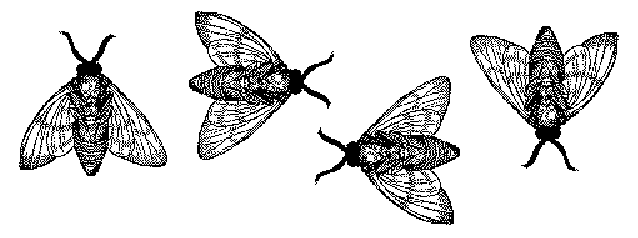
\includegraphics{flies}
\caption{A sample black and white graphic
that needs to span two columns of text.}
\end{figure*}


\begin{figure}

\includegraphics[height=1in, width=1in]{rosette}
\caption{A sample black and white graphic that has
been resized with the \texttt{includegraphics} command.}
\end{figure}

\subsection{Theorem-like Constructs}

Other common constructs that may occur in your article are the forms
for logical constructs like theorems, axioms, corollaries and proofs.
ACM uses two types of these constructs:  theorem-like and
definition-like.

Here is a theorem:
\begin{theorem}
  Let $f$ be continuous on $[a,b]$.  If $G$ is
  an antiderivative for $f$ on $[a,b]$, then
  \begin{displaymath}
    \int^b_af(t)\,dt = G(b) - G(a).
  \end{displaymath}
\end{theorem}

Here is a definition:
\begin{definition}
  If $z$ is irrational, then by $e^z$ we mean the
  unique number that has
  logarithm $z$:
  \begin{displaymath}
    \log e^z = z.
  \end{displaymath}
\end{definition}

The pre-defined theorem-like constructs are \textbf{theorem},
\textbf{conjecture}, \textbf{proposition}, \textbf{lemma} and
\textbf{corollary}.  The pre-defined de\-fi\-ni\-ti\-on-like constructs are
\textbf{example} and \textbf{definition}.  You can add your own
constructs using the \textsl{amsthm} interface~\cite{Amsthm15}.  The
styles used in the \verb|\theoremstyle| command are \textbf{acmplain}
and \textbf{acmdefinition}.

Another construct is \textbf{proof}, for example,

\begin{proof}
  Suppose on the contrary there exists a real number $L$ such that
  \begin{displaymath}
    \lim_{x\rightarrow\infty} \frac{f(x)}{g(x)} = L.
  \end{displaymath}
  Then
  \begin{displaymath}
    l=\lim_{x\rightarrow c} f(x)
    = \lim_{x\rightarrow c}
    \left[ g{x} \cdot \frac{f(x)}{g(x)} \right ]
    = \lim_{x\rightarrow c} g(x) \cdot \lim_{x\rightarrow c}
    \frac{f(x)}{g(x)} = 0\cdot L = 0,
  \end{displaymath}
  which contradicts our assumption that $l\neq 0$.
\end{proof}

\section{Conclusions}
This paragraph will end the body of this sample document.
Remember that you might still have Acknowledgments or
Appendices; brief samples of these
follow.  There is still the Bibliography to deal with; and
we will make a disclaimer about that here: with the exception
of the reference to the \LaTeX\ book, the citations in
this paper are to articles which have nothing to
do with the present subject and are used as
examples only.
%\end{document}  % This is where a 'short' article might terminate



\appendix
%Appendix A
\section{Headings in Appendices}
The rules about hierarchical headings discussed above for
the body of the article are different in the appendices.
In the \textbf{appendix} environment, the command
\textbf{section} is used to
indicate the start of each Appendix, with alphabetic order
designation (i.e., the first is A, the second B, etc.) and
a title (if you include one).  So, if you need
hierarchical structure
\textit{within} an Appendix, start with \textbf{subsection} as the
highest level. Here is an outline of the body of this
document in Appendix-appropriate form:
\subsection{Introduction}
\subsection{The Body of the Paper}
\subsubsection{Type Changes and  Special Characters}
\subsubsection{Math Equations}
\paragraph{Inline (In-text) Equations}
\paragraph{Display Equations}
\subsubsection{Citations}
\subsubsection{Tables}
\subsubsection{Figures}
\subsubsection{Theorem-like Constructs}
\subsubsection*{A Caveat for the \TeX\ Expert}
\subsection{Conclusions}
\subsection{References}
Generated by bibtex from your \texttt{.bib} file.  Run latex,
then bibtex, then latex twice (to resolve references)
to create the \texttt{.bbl} file.  Insert that \texttt{.bbl}
file into the \texttt{.tex} source file and comment out
the command \texttt{{\char'134}thebibliography}.
% This next section command marks the start of
% Appendix B, and does not continue the present hierarchy
\section{More Help for the Hardy}

Of course, reading the source code is always useful.  The file
\path{acmart.pdf} contains both the user guide and the commented
code.

\begin{acks}
  The authors would like to thank Dr. Yuhua Li for providing the
  MATLAB code of the \textit{BEPS} method.

  The authors would also like to thank the anonymous referees for
  their valuable comments and helpful suggestions. The work is
  supported by the \grantsponsor{GS501100001809}{National Natural
    Science Foundation of
    China}{http://dx.doi.org/10.13039/501100001809} under Grant
  No.:~\grantnum{GS501100001809}{61273304}
  and~\grantnum[http://www.nnsf.cn/youngscientists]{GS501100001809}{Young
    Scientists' Support Program}.

\end{acks}
\end{comment}